A four-layer PCB was conceived using Altium Designer and fabricated by PCBWay. It has a size of 50 $\times$ 50 $\times$ 15 mm including the components. The substrate is FR-4 TG150, with spacings of 6mils and a thickness of 1.5mm. The minimum holed size is 0.3mm with tented vias. Finally, the surface finish is HASL with lead with 1oz copper. The 3d-model and final PCB are shown in \autoref{fig:AltiumPCB} and \autoref{fig:PracticalPCB}. 
\begin{figure}[h]
\centering
\begin{subfigure}{0.49\textwidth}
\centering
    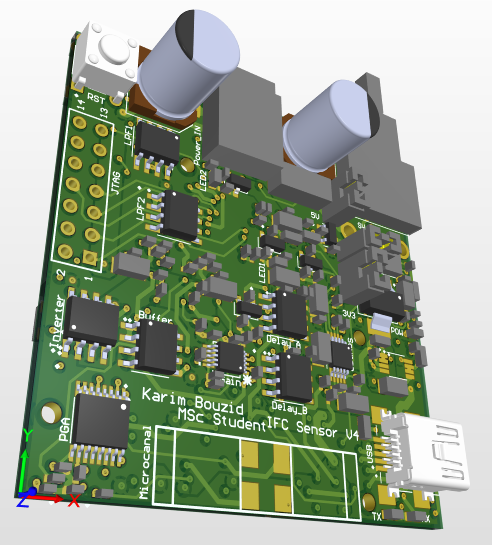
\includegraphics[width=0.9\linewidth]{PCB1}
    \caption{Front view.}
    \label{fig:PCB1}
\end{subfigure}
\begin{subfigure}{0.49\textwidth}
\centering
    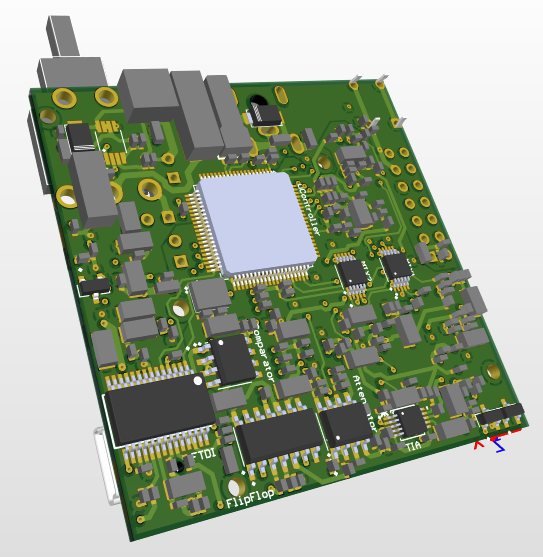
\includegraphics[width=0.96\linewidth]{PCB2}
    \caption{Back view.}
    \label{fig:PCB2}
\end{subfigure}
\caption{3d-model of the back and front views of the PCB as represented in Altium Designer.}
\label{fig:AltiumPCB}
\end{figure}
\begin{figure}[h]
\centering
\begin{subfigure}{0.49\textwidth}
\centering
    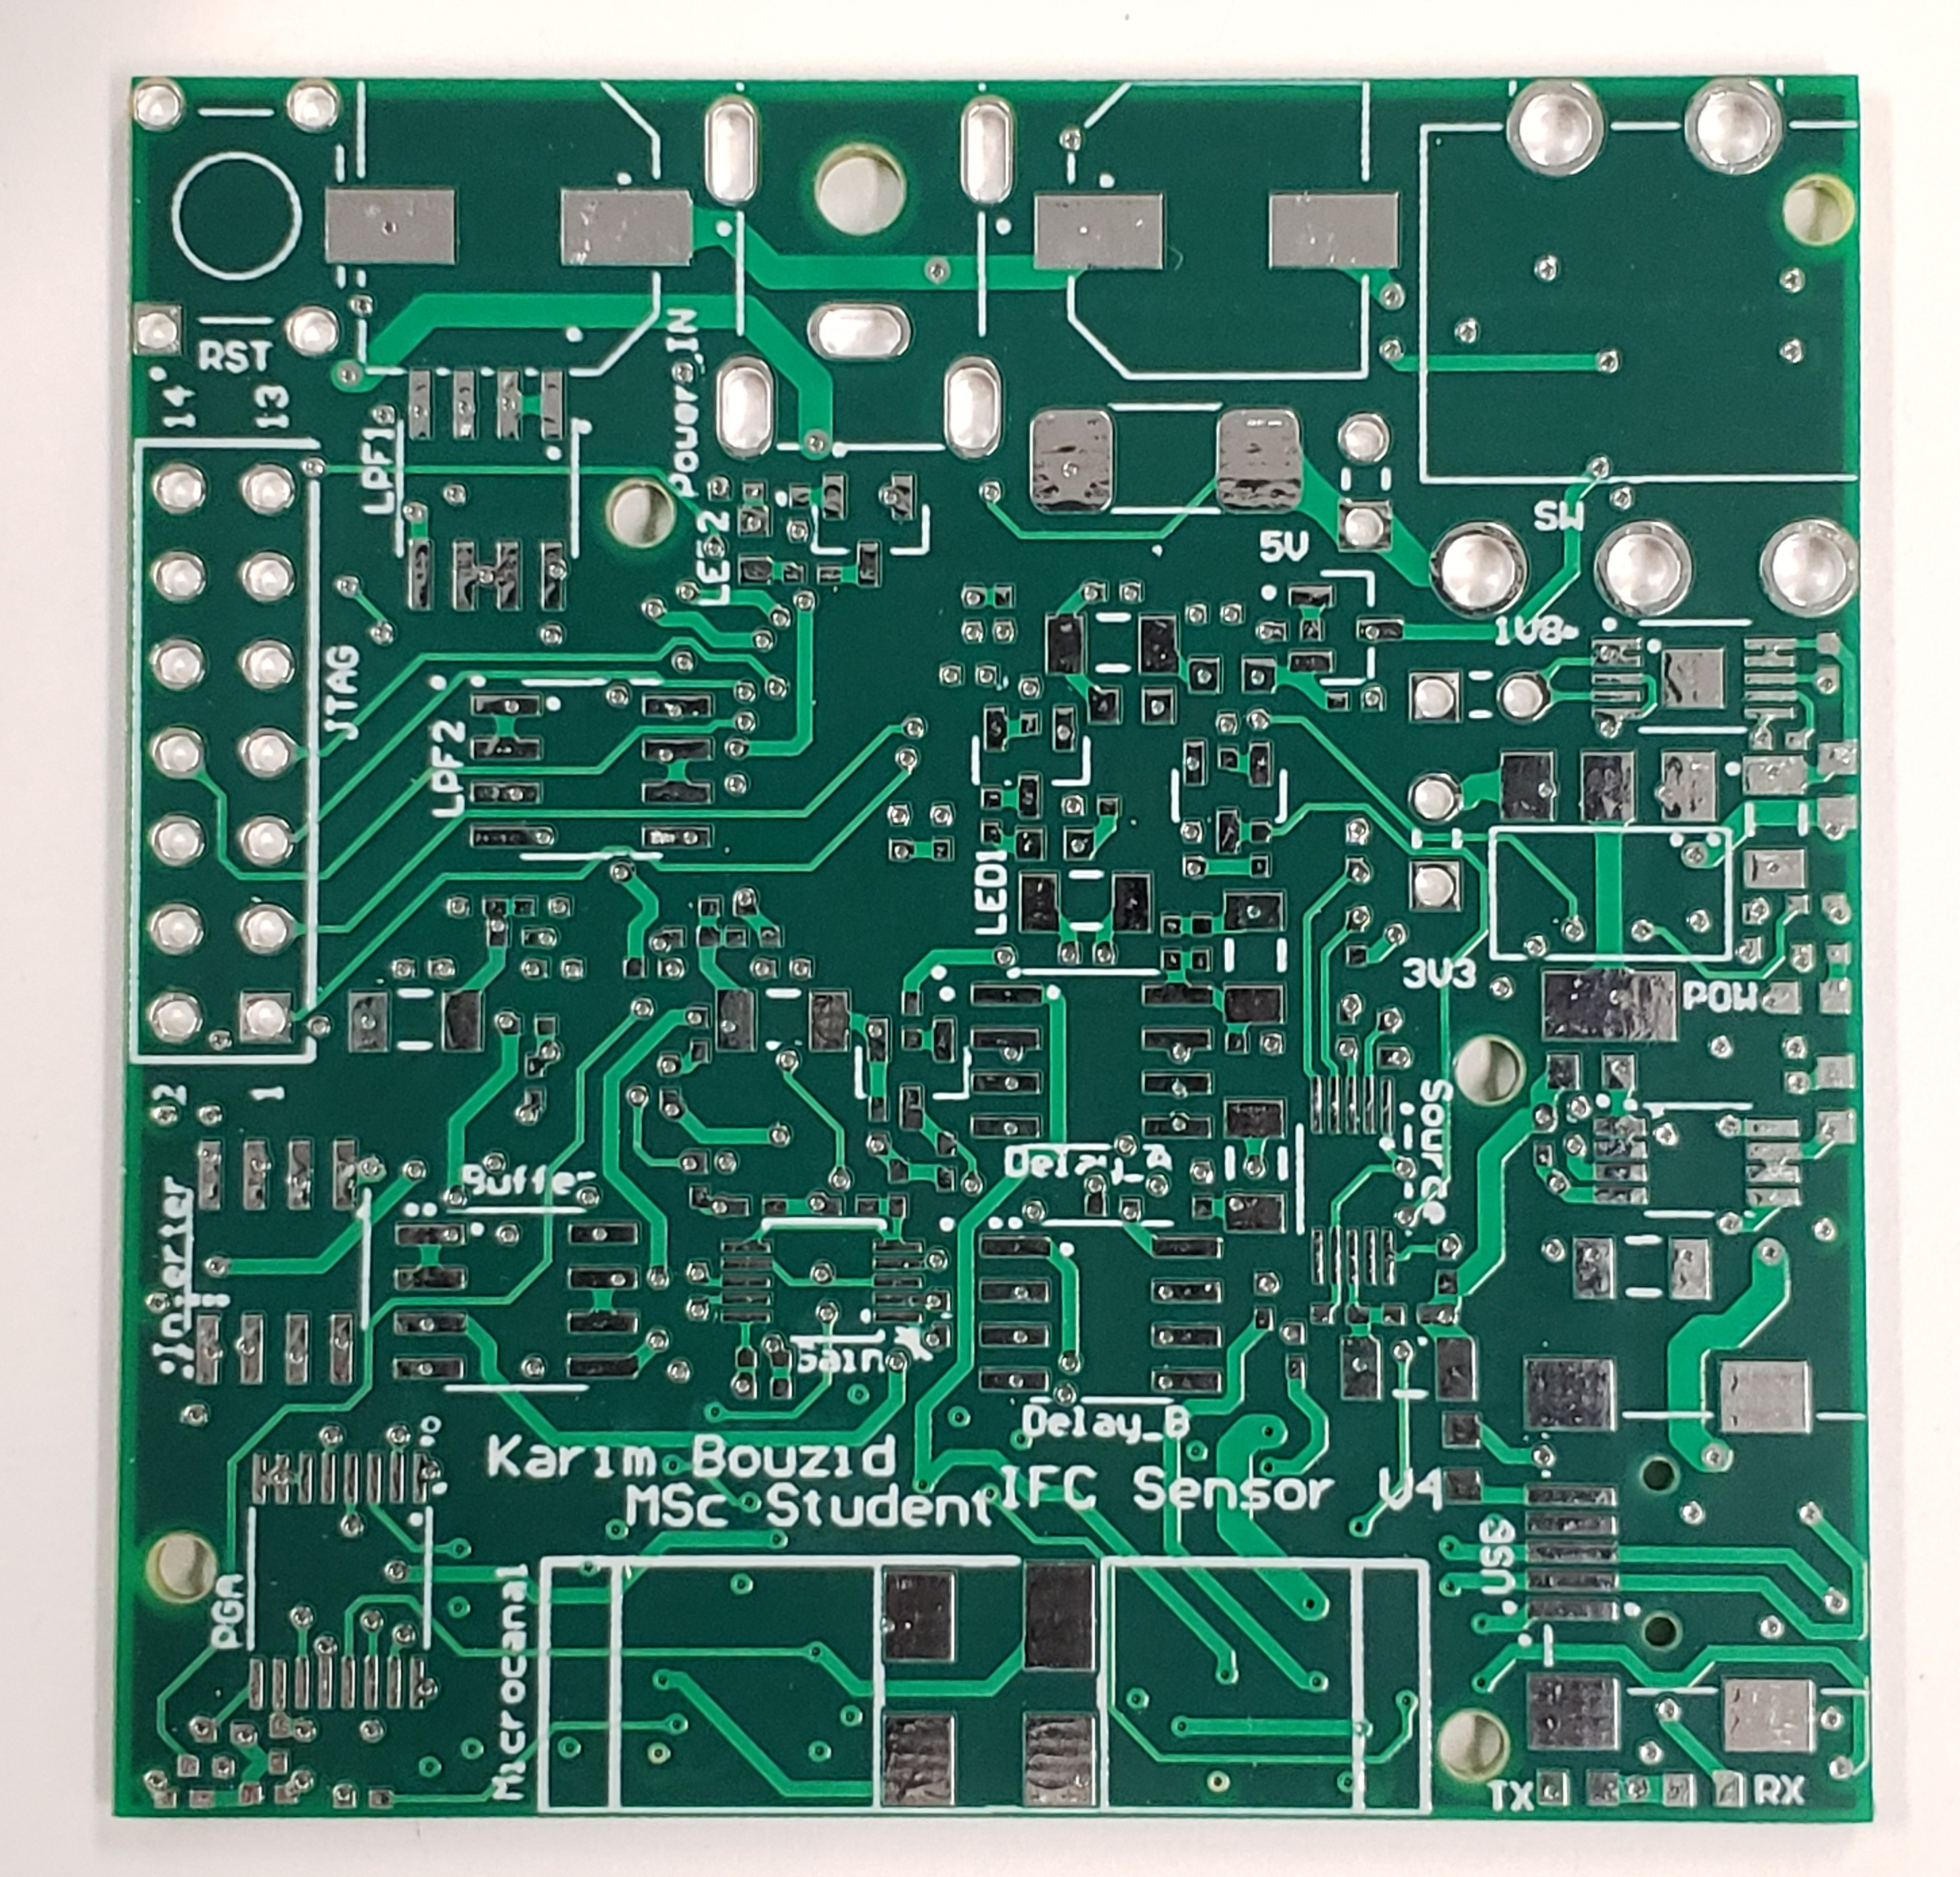
\includegraphics[width=1\linewidth]{BarePCB}
    \caption{Without components.}
    \label{fig:BarePCB}
\end{subfigure}
\begin{subfigure}{0.49\textwidth}
\centering
    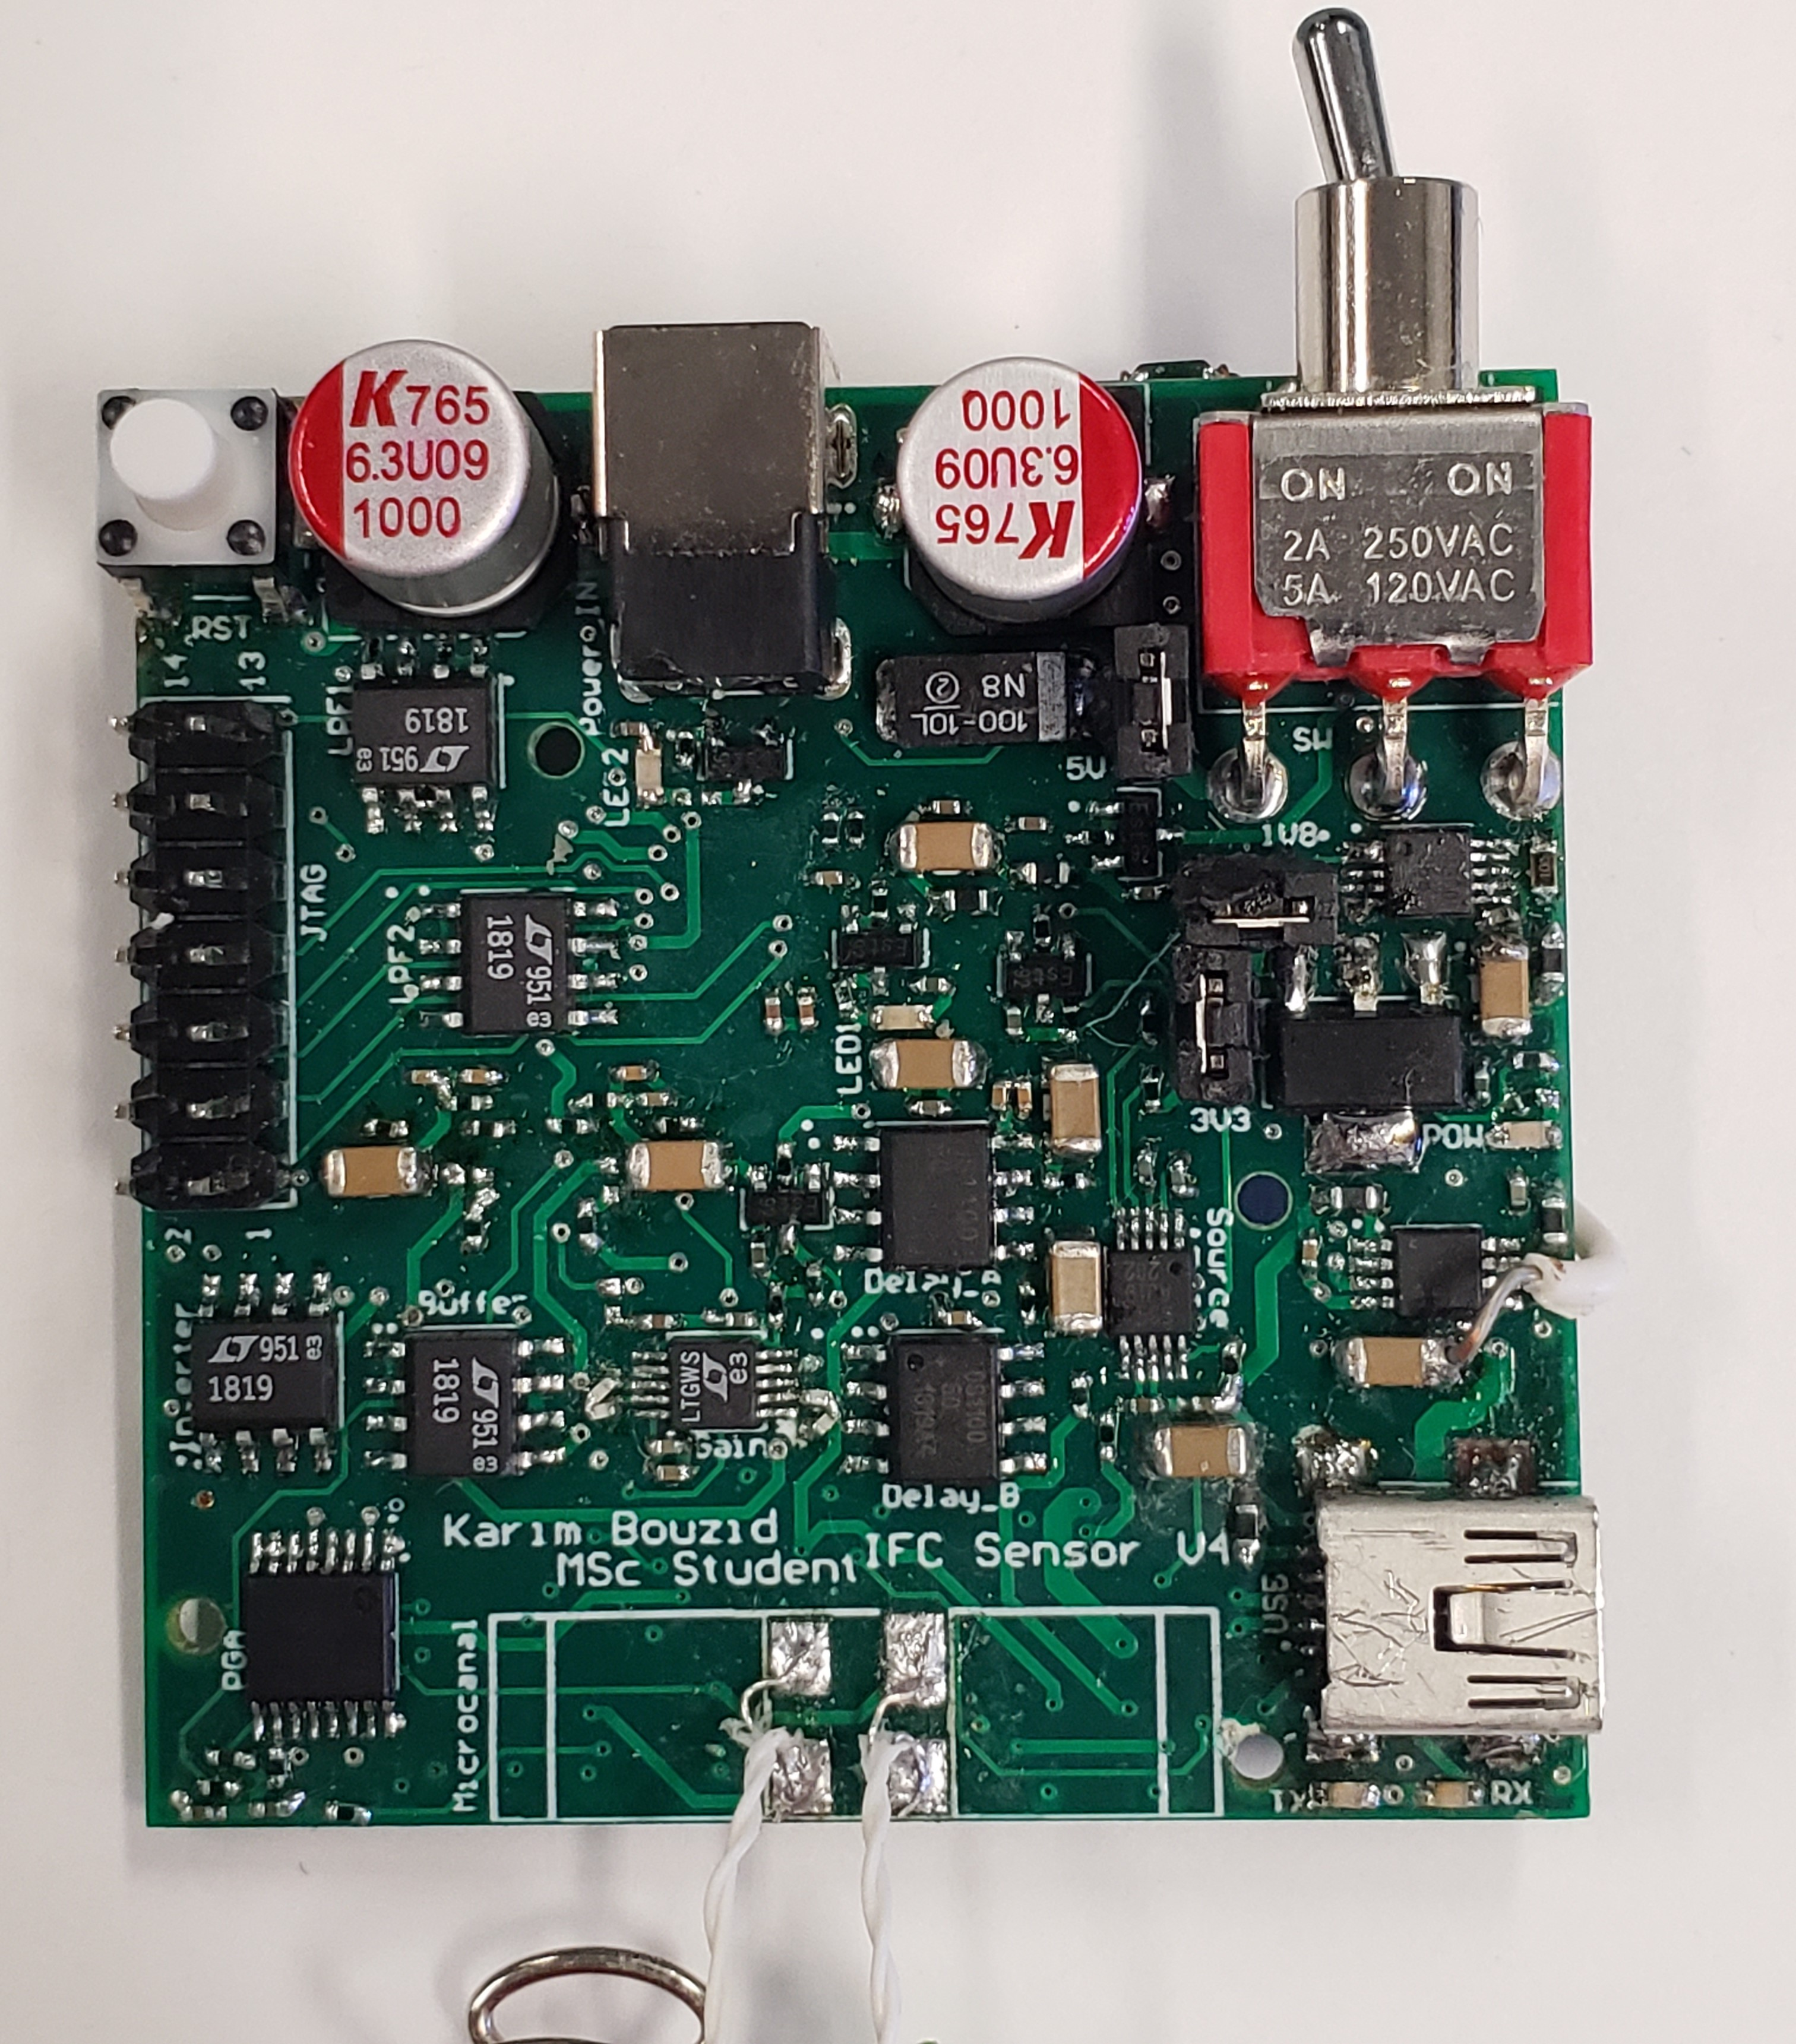
\includegraphics[width=0.85\linewidth]{FunctionalPCB}
    \caption{Soldered components.}
    \label{fig:FunctionalPCB}
\end{subfigure}
\caption{Front-view of the PCB.}
\label{fig:PracticalPCB}
\end{figure}